% ****** Start of file apssamp.tex ******
%
%   This file is part of the APS files in the REVTeX 4.1 distribution.
%   Version 4.1r of REVTeX, August 2010
%
%   Copyright (c) 2009, 2010 The American Physical Society.
%
%   See the REVTeX 4 README file for restrictions and more information.
%
% TeX'ing this file requires that you have AMS-LaTeX 2.0 installed
% as well as the rest of the prerequisites for REVTeX 4.1
%
% See the REVTeX 4 README file
% It also requires running BibTeX. The commands are as follows:
%
%  1)  latex apssamp.tex
%  2)  bibtex apssamp
%  3)  latex apssamp.tex
%  4)  latex apssamp.tex
%
\documentclass[%
 reprint,
%superscriptaddress,
%groupedaddress,
%unsortedaddress,
%runinaddress,
%frontmatterverbose, 
%preprint,
%showpacs,preprintnumbers,
%nofootinbib,
%nobibnotes,
%bibnotes,
 amsmath,amssymb,
 aps,
%pra,
%prb,
%rmp,
%prstab,
%prstper,
%floatfix,
10.5pt,
]{revtex4-1}

\usepackage{graphicx}% Include figure files
\usepackage{subfigure}
\usepackage{multirow}
\usepackage{array}
\usepackage{dcolumn}% Align table columns on decimal point
\usepackage{bm}% bold math
%\usepackage{hyperref}% add hypertext capabilities
%\usepackage[mathlines]{lineno}% Enable numbering of text and display math
%\linenumbers\relax % Commence numbering lines

%\usepackage[showframe,%Uncomment any one of the following lines to test 
%%scale=0.7, marginratio={1:1, 2:3}, ignoreall,% default settings
%%text={7in,10in},centering,
%%margin=1.5in,
%%total={6.5in,8.75in}, top=1.2in, left=0.9in, includefoot,
%%height=10in,a5paper,hmargin={3cm,0.8in},
%]{geometry}

\usepackage{xeCJK}
%\setCJKmainfont[ItalicFont={KaiTi}, BoldFont={KaiTi}]{KaiTi}
\usepackage{textcomp}
\usepackage{chemfig}
\usepackage[version=4]{mhchem}
\usepackage{fontspec}
\usepackage{listings}
\usepackage{xcolor}
\usepackage{xcolor} % 定制颜色
\definecolor{mygreen}{rgb}{0,0.6,0}
\definecolor{mygray}{rgb}{0.5,0.5,0.5}
\definecolor{mymauve}{rgb}{0.58,0,0.82}
\lstset{
backgroundcolor=\color{white},      % choose the background color
basicstyle=\footnotesize\ttfamily,  % size of fonts used for the code
columns=fullflexible,
tabsize=4,
breaklines=true,               % automatic line breaking only at whitespace
captionpos=b,                  % sets the caption-position to bottom
commentstyle=\color{mygreen},  % comment style
escapeinside={\%*}{*)},        % if you want to add LaTeX within your code
keywordstyle=\color{blue},     % keyword style
stringstyle=\color{mymauve}\ttfamily,  % string literal style
frame=single,
rulesepcolor=\color{red!20!green!20!blue!20},
% identifierstyle=\color{red},
language=Mathematica,
}

\usepackage[normalem]{ulem}

\newcommand{\chuhao}{\fontsize{42pt}{44.9pt}\selectfont}    % 初号, 1.5倍行距
\newcommand{\xiaochu}{\fontsize{30pt}{40pt}\selectfont}    % 小初, 1.5倍行距
\newcommand{\yihao}{\fontsize{26pt}{36pt}\selectfont}    % 一号, 1.4倍行距
\newcommand{\erhao}{\fontsize{22pt}{28pt}\selectfont}    % 二号, 1.25倍行距
\newcommand{\xiaoer}{\fontsize{18pt}{18pt}\selectfont}    % 小二, 单倍行距
\newcommand{\sanhao}{\fontsize{16pt}{24pt}\selectfont}    % 三号, 1.5倍行距
\newcommand{\xiaosan}{\fontsize{15pt}{22pt}\selectfont}    % 小三, 1.5倍行距
\newcommand{\sihao}{\fontsize{14pt}{21pt}\selectfont}    % 四号, 1.5倍行距
\newcommand{\sihaox}{\fontsize{14pt}{28pt}\selectfont}    % 四号, 1.5倍行距
\newcommand{\banxiaosi}{\fontsize{13pt}{19.5pt}\selectfont}    % 半小四, 1.5倍行距
\newcommand{\xiaosix}{\fontsize{12pt}{24pt}\selectfont} 	% 小四, 1.5倍行距
\newcommand{\xiaosi}{\fontsize{12pt}{18pt}\selectfont}     
\newcommand{\dawuhao}{\fontsize{11pt}{11pt}\selectfont}    % 大五号, 单倍行距
\newcommand{\wuhao}{\fontsize{10.5pt}{10.5pt}\selectfont}    % 五号, 单倍行距
\newcommand{\xiaowu}{\fontsize{9pt}{9pt}\selectfont}    % 五号, 单倍行距

%\usepackage[fntef]{ctexcap}
%\CTEXsetup[number={\chinese{section}、},format={\Large\bfseries}]{section}
%\setCJKfamilyfont{fangsong}{FangSong}                      %仿宋2312 fs  
%\newcommand{\fangsong}{\CJKfamily{fangsong}}  

\usepackage{wrapfig}
\usepackage{fancyhdr}
\usepackage{fancybox}   


\usepackage{tikz}
\usepackage{circuitikz}



\newcommand{\bra}[1]{\langle #1 |}
\newcommand{\ket}[1]{| #1 \rangle}
\newcommand{\bracket}[2]{\langle #1 | #2 \rangle}
\newcommand{\bracketl}[3]{\langle #1 | #2 | #3 \rangle}
\newcommand{\func}{\mathrm \,}
\newcommand{\define}[2]{
	\begin{definition}
	\begin{description}
	\item[#1]
	#2
	\end{description}
	\end{definition}
}

\newcommand{\sch}{Schr\"odinger}
\newcommand{\grad}{\nabla}
\newcommand{\ueq}{\neq}
\newcommand{\celsius}{\ensuremath{^\circ\hspace{-0.09em}\mathrm{C}}}
\newcommand{\unit}[2]{$#1 \, \mathrm{#2}$}

\begin{document}

%\preprint{APS/123-QED}

\title{The kinetics of the oxidation of formic acid by bromine in aqueous media}% Force line breaks with \\
%\thanks{A footnote to the article title}% give thanks

\author{G. L. Wu}
\affiliation{
	Chemistry Department \\
	Zhejiang University
}


 %\altaffiliation[Also at ]{Physics Department, XYZ University.}%Lines break automatically or can be forced with \\
%\author{Second Author}%
%\email{3160102098@zju.edu.cn}
\author{R. Li, Y. L. Li, Y. X. Qin and Z. W. Huang}
\affiliation{%
 Qiushi science class (chemistry)\\
 Chu Kochen Honor College, Zhejiang University 
}%

%\collaboration{MUSO Collaboration}%\noaffiliation

%\author{Delta Author}
%\affiliation{%
% Authors' institution and/or address\\
% This line break forced with \textbackslash\textbackslash
%}%

%\collaboration{CLEO Collaboration}%\noaffiliation

%\date{\today}% It is always \today, today,
             %  but any date may be explicitly specified

\begin{abstract}

\begin{description}
\item[Keywords]

\end{description}
\end{abstract}

%\pacs{Valid PACS appear here}% PACS, the Physics and Astronomy
                             % Classification Scheme.
%\keywords{Suggested keywords}%Use showkeys class option if keyword
                              %display desired
\maketitle

\tableofcontents

\section{Introduction}
The kinetics of the oxidation of formic acid by bromine in aqueous media has been investigated thoroughly\cite{herbine1980oxidation,brusa1980kinetics}. The total reaction of the oxidation of formic acid by bromine,
\begin{center}
\ce{Br2 + HCOOH ->[k] 2Br- + 2H+ + CO2}
\end{center}
is considered to consist of the following elementary reactions:
\begin{center}
\ce{HCOO- + Br2  ->[k_1] 2 Br- + H+ + CO2} \\
\ce{HCOOH  <=>[K_a] HCOO- + H+} \\
\ce{Br - + Br2  <=>[K_{Br}] Br3-}
\end{center}
Then it follows that
\begin{equation}
	\begin{cases}
	[\ce{HCOO-}] = \frac{K_\text{a}/c(\ce{H+})}{1+K_\text{a}/c(\ce{H+})} c(\ce{HCOOH}) \\[0.3cm]
	[\ce{Br2}] = \frac{1}{1+K_\text{\ce{Br}}/c(\ce{Br-})} c(\ce{Br2})\\[0.3cm]
	\frac{d}{dt} c(\ce{Br2}) = - k_1 [\ce{HCOO-}] [\ce{Br2}] 
	\end{cases}
\end{equation}
if there is abundant supply of \ce{HCOOH} as well as \ce{H+} and \ce{Br-}, the concentration of them can be regarded constant, and the total reaction rate can be written as
\begin{equation}
	\frac{d c(\ce{Br2})}{dt} = -\frac{k_1 K_\text{a}  c(\ce{HCOOH})c(\ce{Br2})/c(\ce{H+})}{[1+K_\text{a}/c(\ce{H+})][1+K_\text{\ce{Br}}/c(\ce{Br-})]}
\end{equation}
and the total reaction rate constant $k$ is equivalent to
\begin{equation}
	k=\frac{k_1 K_\text{a}  c(\ce{HCOOH})/c(\ce{H+})}{[1+K_\text{a}/c(\ce{H+})][1+K_\text{\ce{Br}}/c(\ce{Br-})]}
\end{equation}
Thus the total reaction can be approximated as a reaction in first order, which enables several methods for the detection of the reaction rate constant under different conditions, including spectrophotometric method and electrochemistry method.

The M06-2X functional is a highnonlocality functional with double the amount of nonlocal exchange (2X), and it is parametrized only for nonmetals, which gains a superiority over widely-used functionals including B3LYP, B98, PBE, among calculations involving main-group thermochemistry, kinetics, noncovalent interactions, and electronic excitation energies to valence and Rydberg states.\cite{zhao2008m06}

\section{Methods and Procedures}




\section{Result and Analysis}

\begin{table*}
%\caption{Experimental data of the measurement of $k$ using spectrophotometric method and electrochemistry method respectively, where Group A stands for spectrophotometric method, Group B for electrochemistry method.}
\begin{tabular}{c|ccccc|ccccc}\hline
& \multicolumn{5}{c|}{Group A} & \multicolumn{5}{c}{Group B} \\\hline
\multicolumn{11}{c}{$c(\ce{HCl})$} \\\hline
 $c(\ce{HCl})$/M & 0.08000 & 0.1000 & 0.1200 & 0.1600 & 0.2000 & 0.08000 & 0.1000 & 0.1200 & 0.2000 &\\
 $k \cdot 10^{-3}$/s & 4.252 & 3.491 & 2.829 & 2.159 &
   2.059 & 2.204 & 1.782 & 1.593 & 0.8707 &\\
   $R^2$ & 0.999948 & 0.999963 & 0.999774 & 0.999790 & 0.999584 & 0.999868 & 0.999892 & 0.999863 & 0.999490 &\\\hline
 \multicolumn{11}{c}{$c(\ce{KBr})$} \\\hline
 $c(\ce{KBr})$/M & 0.05000 & 0.07500 & 0.1000 & 0.1500 & 0.2000 & 0.1000 & 0.1200 & 0.2000 & 0.3000 & 0.4000\\
 $k \cdot 10^{-3}$/s &  4.803 & 4.035 & 3.491 & 2.760 & 2.626 & 2.573 & 2.120 & 1.940 & 1.377 & 1.861\\
 $R^2$ & 0.999880 & 0.999937 & 0.999963 & 0.999257 & 0.999954 & 0.999913 & 0.999910 & 0.999715 & 0.999885 &
   0.999706 \\\hline
 \multicolumn{11}{c}{$c(\ce{HCOOH})$} \\\hline
 $c(\ce{HCOOH})$/M & 0.05000 & 0.1000 & 0.1500 & 0.2000 & 0.2500 & 0.03000 & 0.05000 & 0.07000 & 0.1000 & 0.1500 \\
 $k \cdot 10^{-3}$/s & 1.734 & 3.491 & 5.366 & 6.834 & 8.257 & 0.9019 & 1.248 & 1.850 & 2.728 & 3.560 \\
 $R^2$ & 0.999924 & 0.999963 & 0.999956 & 0.999953 &
   0.999883 & 0.999886 & 0.999846 & 0.999843 & 0.999938 &
   0.999907\\\hline
 \multicolumn{11}{c}{$T$} \\\hline
 $T/\celsius$ & 25.00 & 30.00 & 35.00 & 40.00 & 45.00 & 25.00 & 30.00 & 35.00 & 40.00 & 45.00\\
 $k \cdot 10^{-3}/s$ &  3.491 & 5.426 & 8.001 & 11.47 & 15.15 & 1.850 & 3.104 & 4.981 & 8.234 & 12.49 \\
 $R^2$ & 0.999963 & 0.999928 & 0.999431 & 0.999916 &
   0.999844 & 0.999843 & 0.999913 & 0.999936 & 0.999683 &
   0.999425 \\\hline
\end{tabular}
\end{table*}

\begin{figure*}
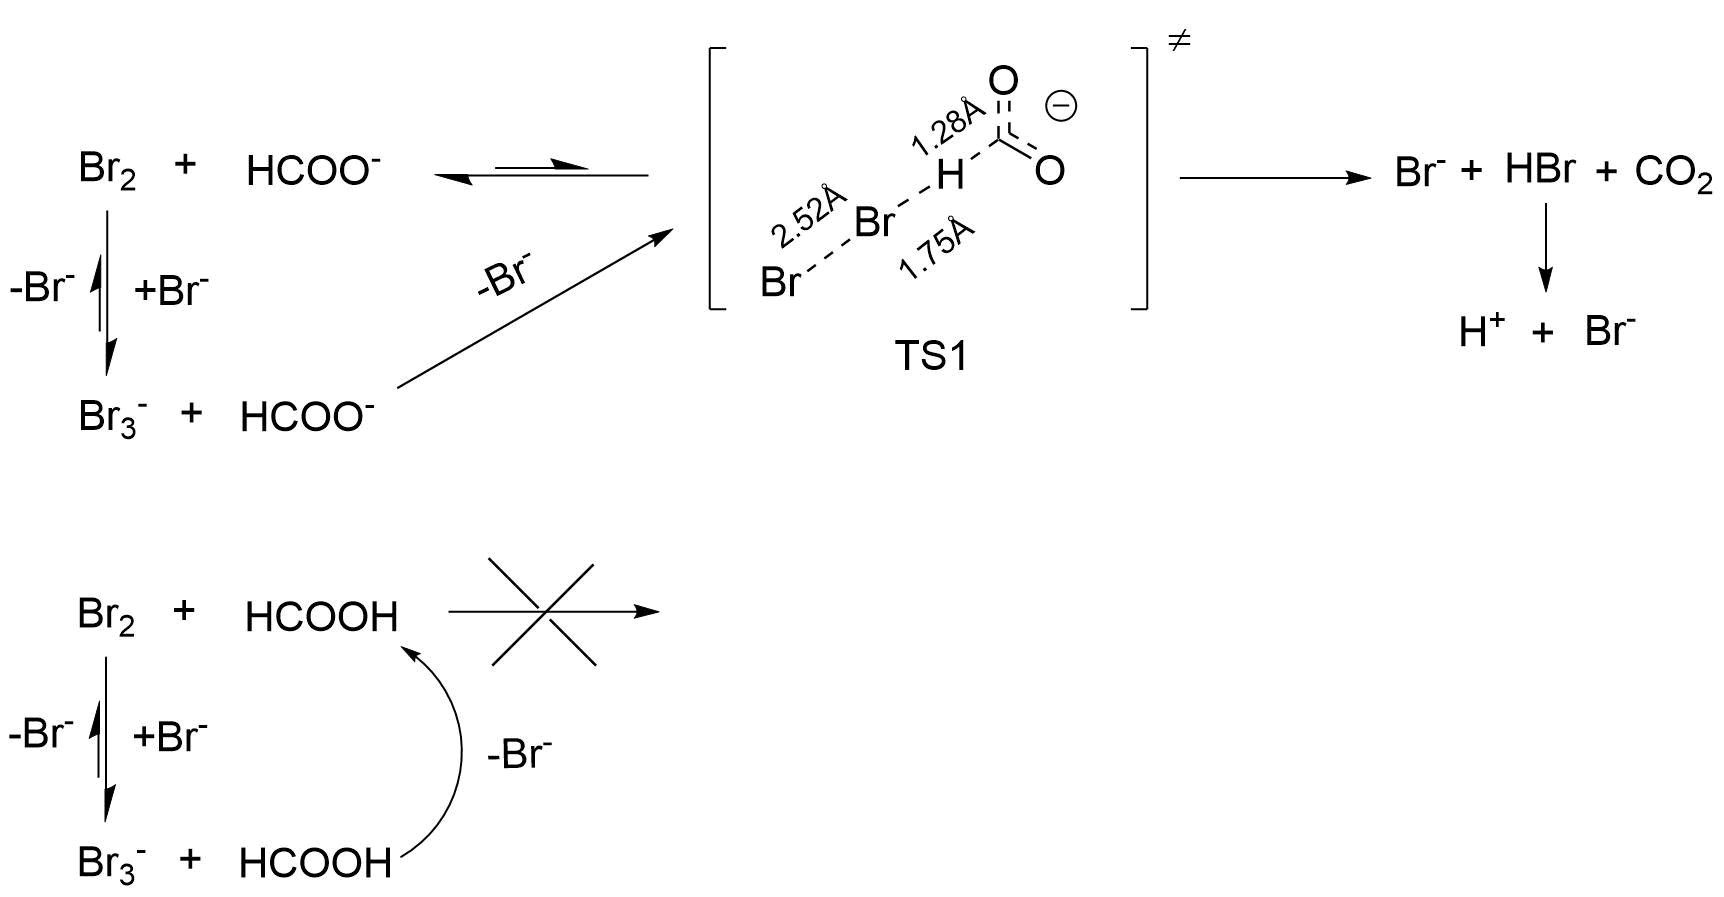
\includegraphics[width=0.8\textwidth]{figures/reaction_mechanic.png}
\caption{The proposed mechanism of the oxidation of formic acid by bromine}
\end{figure*}

\begin{table*}
\centering
\caption{Calculation result from Gaussian 16 of the energy / Gibbs free energy (without solvent effect) of the \ce{HCOO-}-\ce{Br2}~system in different distance between hydrogen atom in formic acid and bromide atom in bormine, choosing -5337 Hartree as the zero potential energy surface. "N/A" refers to unavailability of the data, due to the fact that the system did not converge during the calculation.}
\begin{tabular}{ccccccccccc}\hline
Distance(\AA) & 1.9 & 2.0 & 2.1 & 2.2 & 2.4 & 2.6 & 2.8 & 3.1 & 3.5 & 5.0 \\\hline
-E(Hartree) & .537892 & .533230 & .529462 & .526210 & .520616 & .516360 & .512932 & .508763 &.504027 & .498300 \\
-G(Hartree) & .555580 & .549755 & .545271 & .541625 & .535825 & .531732 & .528610 & .524980 & N/A & .525179 \\\hline
\end{tabular}
\end{table*}

\begin{table*}
\centering
\caption{Calculation result from Gaussian 16 of the Gibbs free energy of different species in the system, with solvent effect considered.}
\begin{tabular}{ccccccccc}\hline
Species & \ce{Br2} & \ce{Br-} & \ce{Br3-} & \ce{HBr} & \ce{H+} & \ce{HCOOH} & \ce{HCOO-} & \ce{CO2} \\
-G(Hartree) & -5148.359998 & -2574.362887 & -7722.741404 & -2574.787315 & -0.22518 & -189.721106 & -189.279246 & -188.553856 \\\hline
\end{tabular}
\end{table*}

\begin{equation}
	\frac{d c_s}{dt} = k (c_l - c_s)
\label{diffusion}
\end{equation}
where $c_l$ refers to the concentration of the substance in the liquid phase, while $c_s$ the concentration in the solid phase. Considering that the diffusion of the substance is comparatively small, $c_l$ can be regarded as dominated by chemical reaction, namely
\begin{equation}
	c_l = c' e^{-k't}
\end{equation}
where $c',k'$ are constants. (\ref{diffusion}) can be deduced by assuming the form of $c_s$ as
\begin{equation}
	c_s = \chi(t) e^{-k't}
\end{equation}
which gives
\begin{equation}
\begin{cases}
	\chi(t) = C_1 e^{(k'-k) t} + C_2,\\
	 c_s = \frac{k c'}{k'-k} e^{-k't}(e^{(k'-k)t}-1)
	 \end{cases}
\end{equation}
where $C_1,C_2$ are constants that are replaced using the boundary condition,
\begin{equation}
	c_s \big|_{t=0} = 0
\end{equation}
and infomation from $c_s$.
It reveals the influence of the diffusion in the measurement, the term $e^{(k'-k)t}-1$ being the main delimiter. Smaller $k$ with small sets of $t$ will result in larger deficiency in the measurement of $k'$, which might be the case in the electrochemistry method.

The non-constant response function of the measurement system might also contribute to the error. The detection of current is achieved through complicated electromagnetic system, which results in non-constant response function. The output function can be regarded as the convolution of the signal function and the response function, namely
\begin{equation}
	P = S * R = \int S(t) R(T-t) \, dt
\end{equation}
where $P$ stands for the output, while $S$ and $R$ for the signal function and the response function, with $T$ defined as the time interval for a measurement. Given that $S$ is a exponential function, it can be readily proved that $P$ is also a exponential function under the same base. A non-constant response function, however, deviates the output function with considerable error, and it is conspicuous that a larger time interval leads to worse data sets. Compared with spectrophotometric method, electrochemistry method is much more likely to suffer from such a factor, w.r.t. its relatively longer measurement of time.




\bibliography{References}
\end{document}
